%TODO:


\documentclass[draft]{scrartcl}


\usepackage[utf8]{inputenc}
\usepackage[english]{babel}
\usepackage{lmodern} 
\usepackage[T1]{fontenc}
\usepackage{booktabs}
\usepackage{multirow}
\usepackage{wrapfig}


% PAKETE
\usepackage{siunitx}
\usepackage{graphicx}
\usepackage[usenames,dvipsnames]{xcolor}
\usepackage{placeins}
\usepackage{longtable}
\usepackage{enumitem}
\usepackage{bbm}

\usepackage{amssymb} % math symbols
\usepackage{amsmath} % ams
\usepackage{amsfonts} % mathmatical fonts

% caption indenting
 \usepackage[format=plain,indention=0em,labelfont=bf,margin=1em]{caption} 
 \usepackage{subfig} %subfigures ^^
\usepackage[protrusion=true,expansion=true]{microtype} % denser font, "-" behind line
\usepackage{esint} % nicer double and triple integrals
\usepackage{fancyhdr} % fancy headers
\usepackage[colorlinks=true,linkcolor=black,citecolor=black,filecolor=black,urlcolor=black]{hyperref}



% EINSTELLUNGEN
\sisetup{seperr,repeatunits=false}
\numberwithin{equation}{section}
\numberwithin{figure}{section}
\numberwithin{table}{section}

% EIGENE FUNKTIONEN
\newcommand{\re}{\operatorname{Re}}
\newcommand{\im}{\operatorname{Im}}
\newcommand{\gquote}[1]{\glqq #1 \grqq}

\newcommand{\eq}[2]{\begin{equation}#1\label{#2}\end{equation}}
\newcommand{\eqand}[0]{\hspace{.25cm} \bigwedge \hspace{.25cm}}
\newcommand{\grafik}[2]{\begin{figure}[h]\centering \includegraphics[width=10cm]{#1.eps}  \caption{#2} \label{#1} \end{figure} }
\newcommand{\grafikq}[3]{\begin{figure}[h]\centering \includegraphics[width=10cm]{#1.eps}  \caption[#2]{#3} \label{#1} \end{figure} }
\newcommand{\tbl}[3]{\begin{table}[h]\caption{#1}\label{#2}\begin{center}#3\end{center}\end{table}}
\newcommand{\Abbildung}[1]{\textsl{Abbildung \ref{#1}}}
\newcommand{\AbbildungI}[1]{\textsl{(Abbildung \ref{#1})}}
\newcommand{\Tabelle}[1]{\textsl{Tabelle \ref{#1}}}
\newcommand{\TabelleI}[1]{\textsl{(Tabelle \ref{#1})}}
\newcommand{\Formel}[1]{(\ref{#1})}
\renewcommand{\d}{\mathrm{d}}
\newcommand{\ve}[1]{\mathbf{ #1} }

\title{Ma 5: Dynamical Processes in Lipid Membranes}
\subtitle{Tutor: Dr. P. Chernev}
\author{Benjamin Huber, Carolin Wille}
\date{January 30, 2012}

\begin{document}
\thispagestyle{empty}
\maketitle
\tableofcontents
\clearpage

\section{Introduction}
In this experiment blabla


\subsection{Fluorescence and Absorption spectra}
\subsubsection{Dipole Transitions and the Franck-Condon Principle}
In order to understand the emission and absorption spectrum of molecules, it is important to know the structure of energy levels and the transitions, which can occur between them. In the Born-Oppenheimer approximation, which is valid if the electronic transitions happen on a much shorter time scale than the changes in the distance of the atomic nuclei, the wavefunction, which describes the state of the molecule factorises in electronic and nuclear components. The components connected to the nuclei include rotation and vibrational states. If the rotational degrees of freedom are suppressed, e.g. if the molecule is embedded in a certain structure, only the vibrational levels are relevant. The transitions, which lead to the emission of visible light are electronic transitions, that are combined with a vibronic transition. In the dipole approximation, that is valid if the wavelength of the emitted light is considerably longer than the atomic radii, the probability amplitude for such an electronic-vibronic transition is given by the matrix elements of the final and initial states $\Psi,\Psi'$ with the dipole operator $\ve {\hat{D}}$
\eq{ P = \langle \Psi'  \mid   \ve {\hat{D}} \mid \Psi \rangle =  \langle \psi_\text{el'} \mid   \ve {\hat{D}_{el}} \mid \psi_\text{el} \rangle \langle \psi_\text{s'} \mid \psi_\text{s} \rangle \langle \psi_\nu'  \mid  \psi_\nu \rangle \; .} {transition }
The spatial overlap of the two vibronic state nuclear wavefunction squared  $\lvert \langle \psi_\nu'  \mid  \psi_\nu \rangle \rvert ^2$ is called the Franck-Condon factor and expresses the fact, that transitions are more likely to occur, if the position of the nuclei remain more or less the same during an electronic transition. This is called the Franck-Condon principle and is illustrated in figure \ref{condon}. 
The direction of the dipole operator gives the polarization direction of the photons, which are absorbed or emitted.
Considering two electronic states with similar vibronic structure, the absorption spectrum is symmetric to the fluorescence spectrum as a consequence of the Franck-Condon principle (cf. \ref{condon}). This symmetry can be detected in the experiment although the equal spacing of the energy levels is an idealization, meaning that the real structures do not look exactly symmetric.

\subsubsection{Relaxation Processes}
An excited state can relax into its groundstate via different intermediate processes. Radiation less transitions, which can occur via exchange of phonons or collisions with other atoms and molecules are usually very fast, because the energy difference between those states is typically small. Thus, an excited vibronic state decays fast into its ground state. The relaxation of the electronic excited state and vibronic ground state into the electronic ground state and excited vibronic state (cf. fig \ref{condon} \textbf{(c)}) is called fluorescence. As its emitted photons are typically in the visible light regime, fluorescence is a luminescent process. The other luminescence, which can occur is phosphorescence, where the system decays first into a state, which is forbidden according to spin selection rules. Such a transition, where the electron spin changes is called intersystem crossing. The decay into ground state is again forbidden according to the dipole selection rules. Therefore, the lifetime if this state is very high, which leads to the phenomenon of light emission long after absorption.

Another process is the so called fluorescence quenching, where the fluorescence is suppressed by the transition of energy to certain molecules. For the molecule used in the experiment, water acts as a quenching molecule and reduces the fluorescence intensity to $1/200$ of the value in hydrophobic media like the interior of lipid membrane bilayers.

The fluorescence lifetime $\tau_f$ is defined as the inverse of the decay rate $k_f$, which characterises the exponential decay of the excited state via fluorexcence
\eq{N(t) =N_0 \exp (-k_f \cdot  t) , \qquad \tau_f=1/k_f \; .}{rate}



\subsubsection{Specifications to Fluorophores}
In heterocyclic and aramoatic molecules, which are called fluorophores, the ground state is given, when the electrons are both in bonding $\pi$ orbitals. They have antiparallel spins leading to total spin zero, which is referred to as a singulet state S$_{0,\pi\pi}$. The first excited electronic state is then a state, where one electron is in the antibonding $\pi^*$ orbital. In this excited state, the electrons can have parallel or antiparallel spin leading to singulet S$_{1, \pi \pi^*}$ and triplet states T$_{1, \pi \pi^*}$. The triplet states have usually lower energy.

In this experiment the fluorophore Diphenylhexatriene (DPH) is used as a reporter probe, which is embedded in to the lipid membrane.

\begin{figure}
\centering
\subfloat[][Franck-Condon Principle]{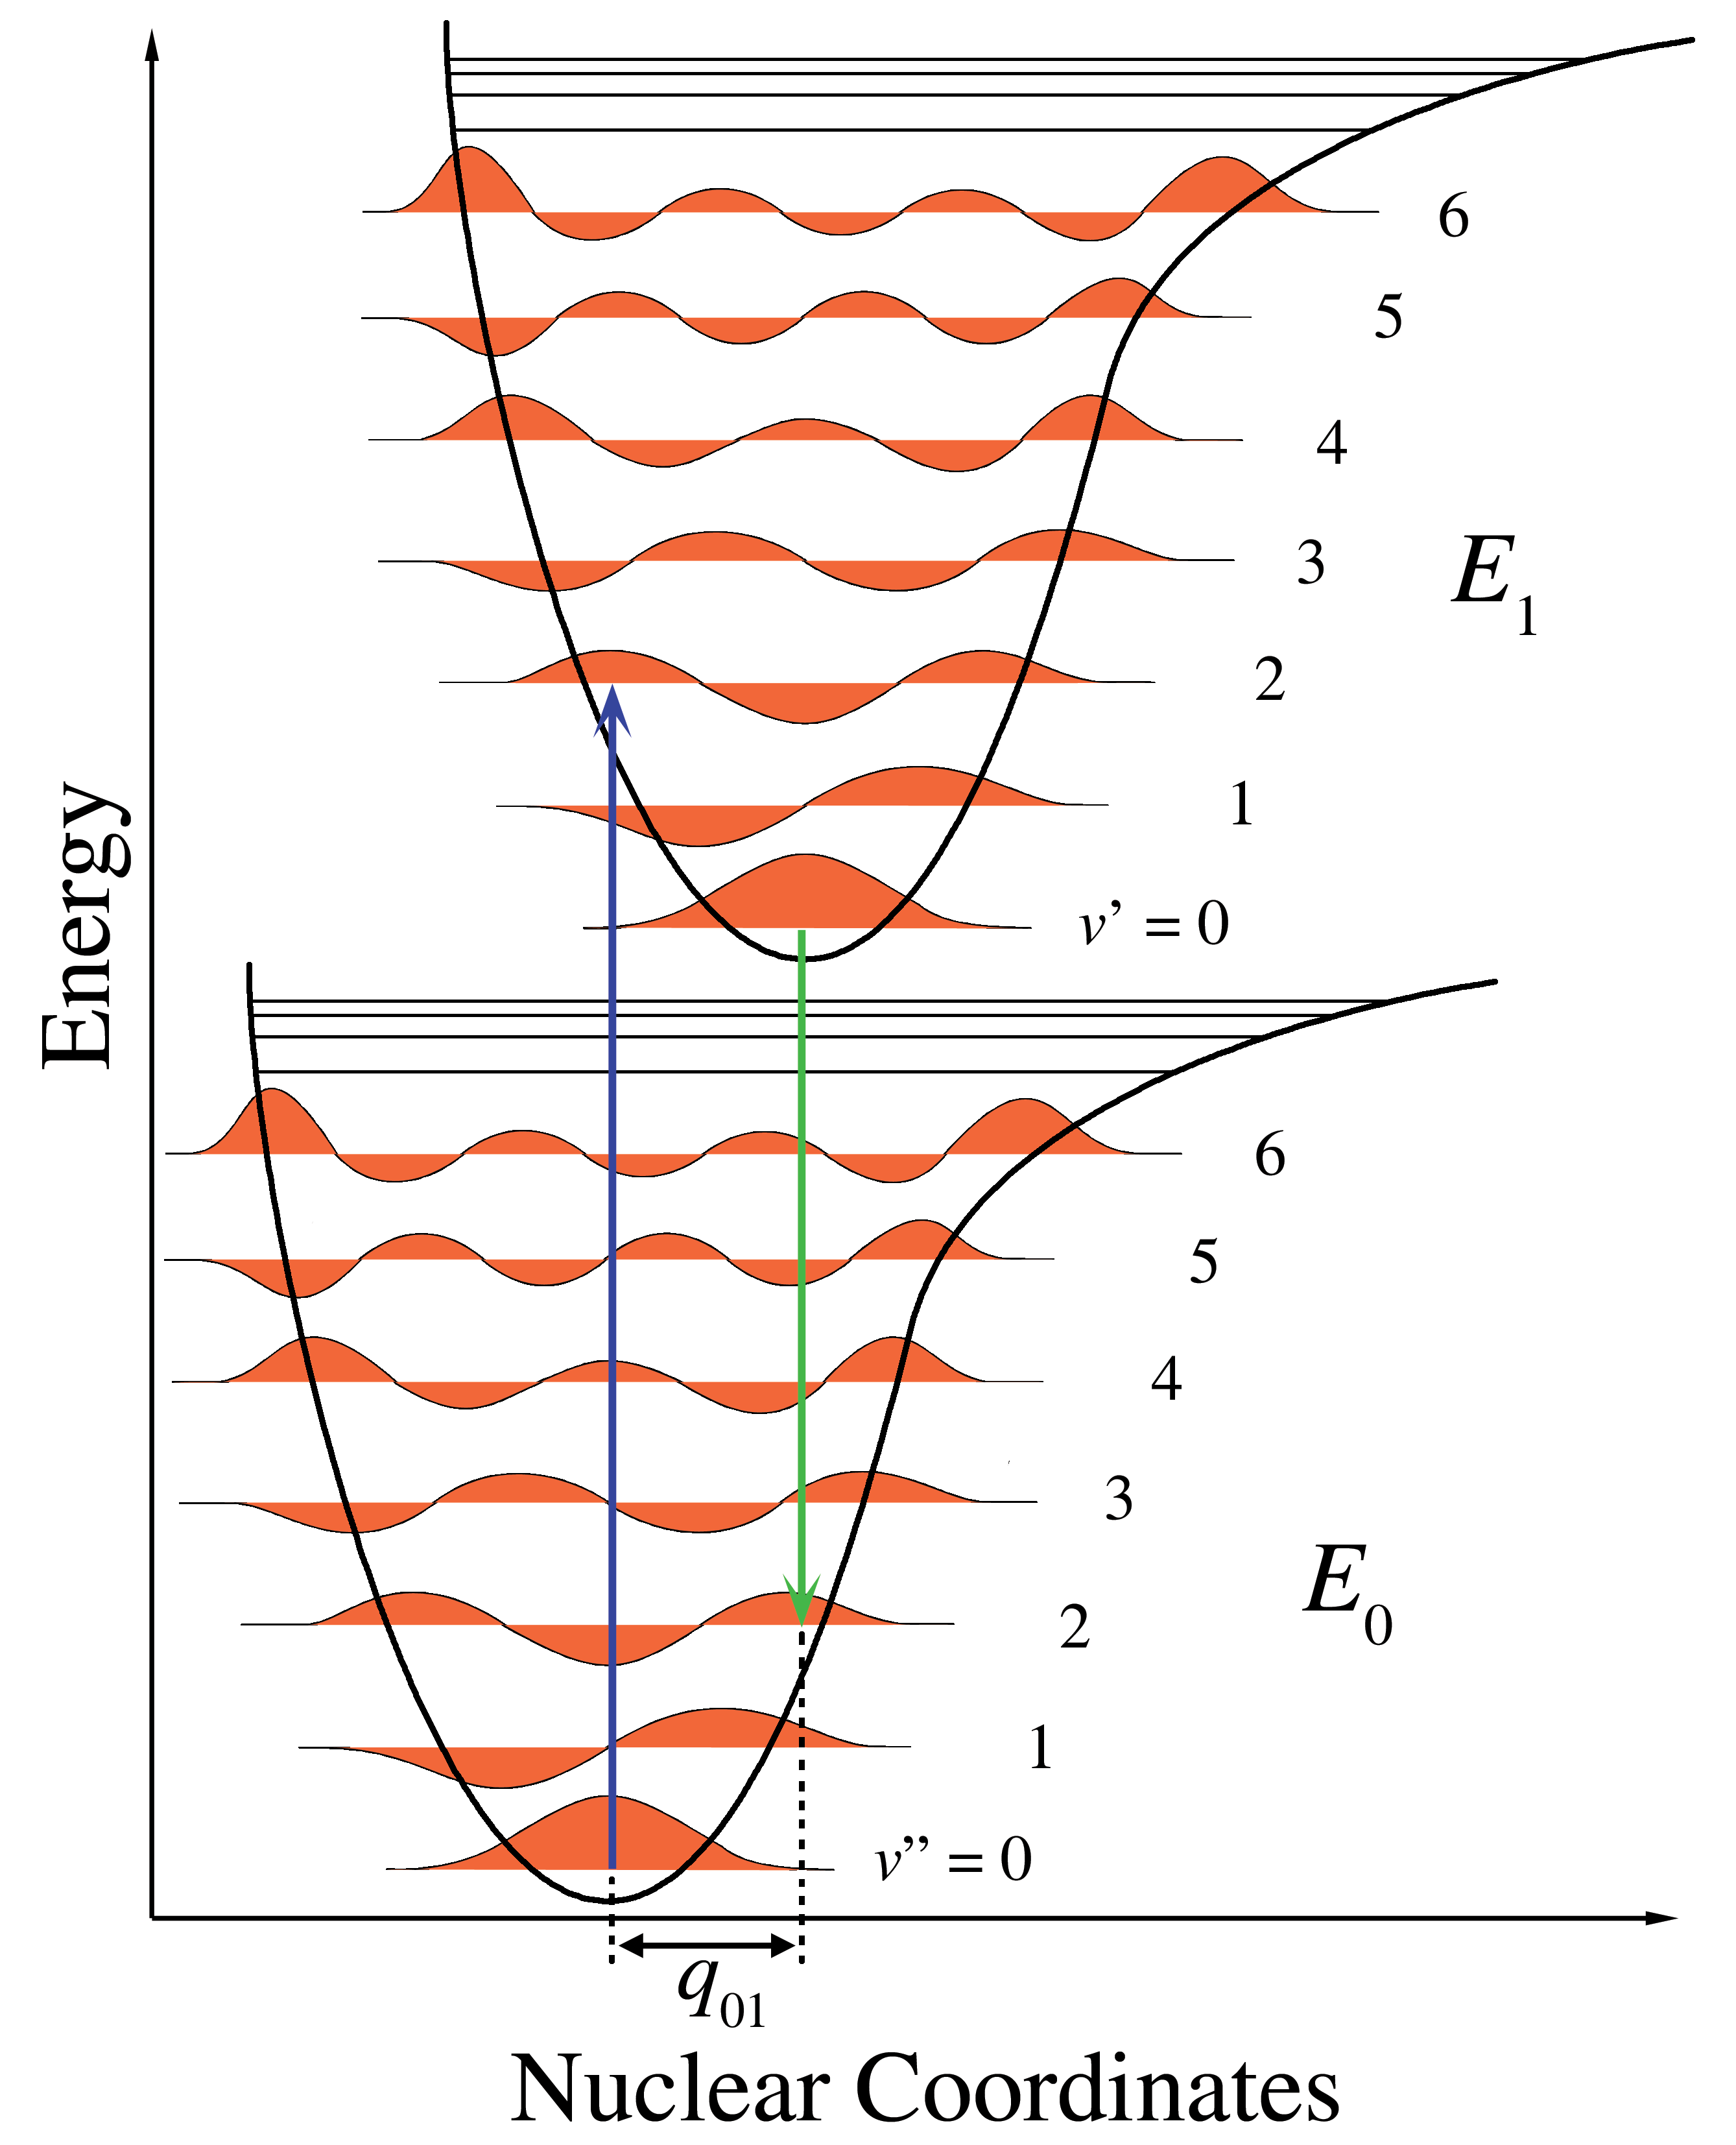
\includegraphics[width=0.5\linewidth]{img/condon.png}}
\hfill
\subfloat[][Spectrum]{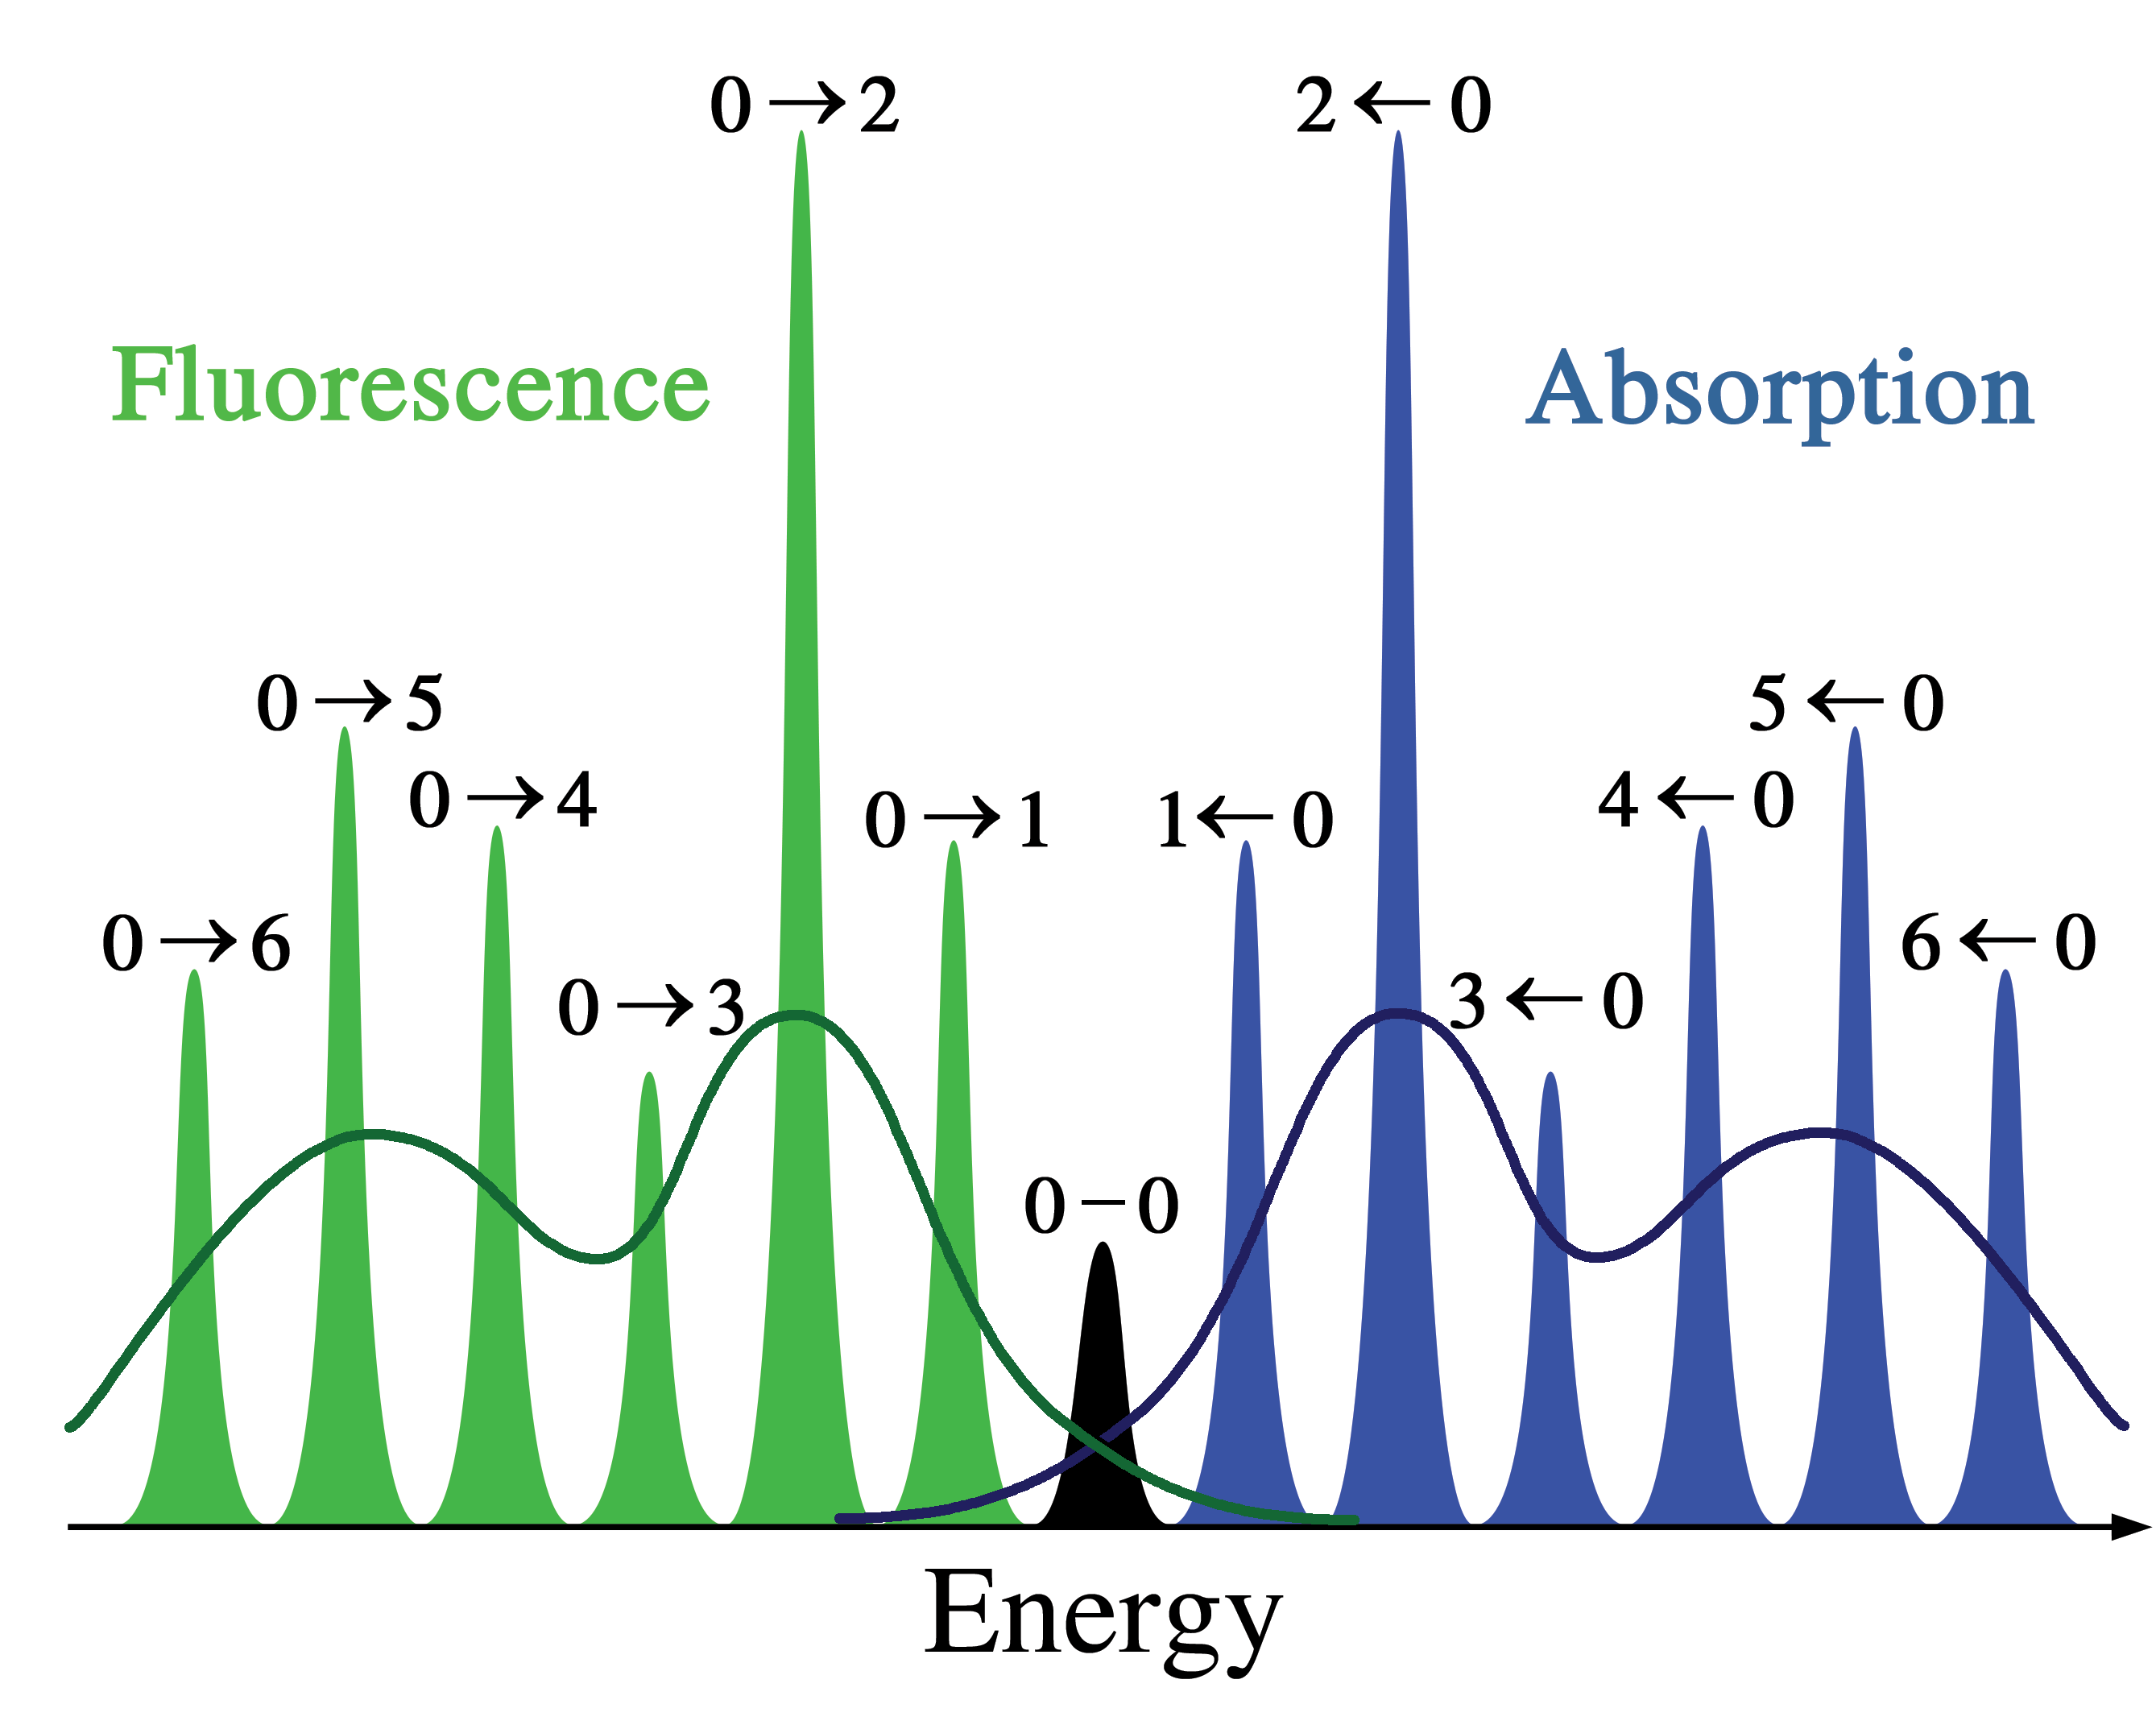
\includegraphics[width=0.5\linewidth]{img/absorptionemission.png}}

\subfloat[][Jablonski Diagram]{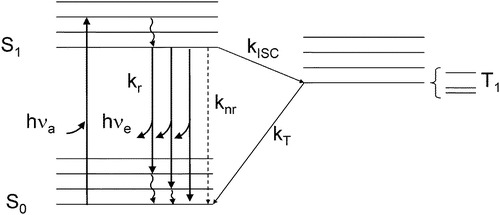
\includegraphics[width=0.7\textwidth]{img/Jablonski.jpg}}
\caption{ \small \textbf{(a)} Illustration of the Franck-Condon principle, which is a direct consequence of the Born-Oppenheimer approximation and states, that those electronic-vibraonic transitions are favored, which leave the inter-nuclei distance mostly unchanged. 
\textbf{(b)} Symmetric structure of an absorption and fluorescence spectrum. Sharp peaks will be visible in dilute gases, while in liquids and solids the peaks are widened. 
\textbf{(c)} Jablonski Diagram of different relaxation processes. ISC denotes intersystem crossing. $K_T$ the relaxation via phosphorescence. $K_r$ denotes fluorescence and $K_{nr}$ radiationless transitions, which also reduce the fluorescence lifetime. \footnotesize Source: \textbf{(a)}, \textbf{(b)} \url{http://en.wikipedia.org/wiki/Franck-Condon_principle}, \textbf{(c)} \cite{omg}}
\label{condon}
\end{figure}








\clearpage
 \bibliographystyle{unsrt}
\bibliography{bib}



\end{document}


